\documentclass[border=4pt]{standalone}
\usepackage{amsmath,amssymb,tikz}
\usetikzlibrary{arrows.meta,calc}
\definecolor{figB}{RGB}{31,90,166}\definecolor{figR}{RGB}{176,48,48}\definecolor{figG}{RGB}{46,125,50}\definecolor{figO}{RGB}{214,120,20}
\begin{document}
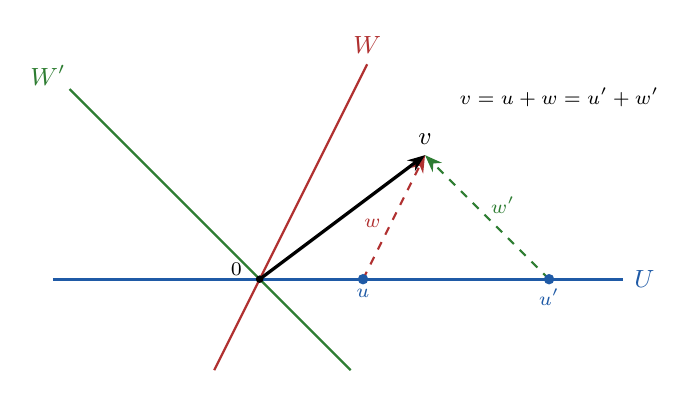
\begin{tikzpicture}[scale=1.05,>={Stealth[length=2.2mm]}]
\draw[figR,thick] (-0.55,-1.1)--(1.3,2.6) node[above,font=\small]{$W$};
\draw[figG,thick] (1.1,-1.1)--(-2.3,2.3) node[above left,font=\small,inner sep=1pt]{$W'$};
\draw[figB,very thick] (-2.5,0)--(4.4,0) node[right,font=\small]{$U$};
\coordinate (v) at (2,1.5); \coordinate (u) at (1.25,0); \coordinate (u2) at (3.5,0);
\draw[->,figR,thick,dashed] (u)--(v) node[pos=0.45,left,font=\scriptsize]{$w$};
\draw[->,figG,thick,dashed] (u2)--(v) node[pos=0.5,above right,font=\scriptsize,inner sep=1pt]{$w'$};
\draw[->,very thick] (0,0)--(v) node[above,font=\small]{$v$};
\fill[figB] (u) circle (1.8pt) node[below,font=\scriptsize]{$u$};
\fill[figB] (u2) circle (1.8pt) node[below,font=\scriptsize]{$u'$};
\fill (0,0) circle (1.3pt); \node[font=\scriptsize] at (-0.28,0.12) {$0$};
\node[font=\scriptsize,anchor=west] at (2.3,2.2) {$v=u+w=u'+w'$};
\end{tikzpicture}
\end{document}
